Cloud Computing has emerged as an attractive platform for increasingly
diverse compute- and data-intensive applications, as it allows for
low-entry costs, on demand resource provisioning and allocation, and
reduced cost of maintaining internal IT
infrastructure~\cite{tchana_cits_2012}. %Cloud computing will continue
%to grow and attract attention from commercial and public market
%segments. Recent studies predict annual growth rate of 17.7 percent by
%2016, making cloud computing the fastest growing segment in the
%software industry.
As the demand for cloud computing
accelerates, cloud service providers (CSPs) will be faced with the
need to expand their underlying infrastructure to ensure the expected
levels of performance and cost-effectiveness, resulting
in a multi-fold increase in the number of computing, storage and
communication components in their datacenters. The direct implication of large datacenters is increased management complexity and propensity to
failure.

Failure to deliver
the service as specified subjects the CSP to a loss of revenue. In addition, CSPs face rising energy costs of their large-scale
datacenters. This raises the question of how
fault tolerance might impact power consumption and ultimately the
expected profit of the service providers. In this work, we address the above challenge 
by studying the application of Shadow Replication for QoS in cloud computing.

\section{Cloud workload characteristics}

Cloud computing workload ranges from business applications and
intelligence, to analytics and social networks mining and log
analysis, to scientific applications in various fields of sciences and
discovery. These applications exhibit different behaviors, in term of
computation requirements and data access patterns. While some
applications are compute-intensive, others involve the processing of
increasingly large amounts of data. The scope and scale of these
applications are such that an instance of a job running one of these
applications requires the sequential execution of multiple computing
phases; each phase consists of thousands, if not millions, of tasks
scheduled to execute in parallel and involves the processing of a very
large amount of data~\cite{lin2010data,Ferdman:2012:CCS:2150976.2150982}. This
model is directly reflective of the \emph{MapReduce} computational
model, which is predominately used in
Cloud Computing \cite{mrbs}.  An instance of this model, is depicted in Figure \ref{fig:system_model}.


\begin{figure}[!h]
	\begin{center}
		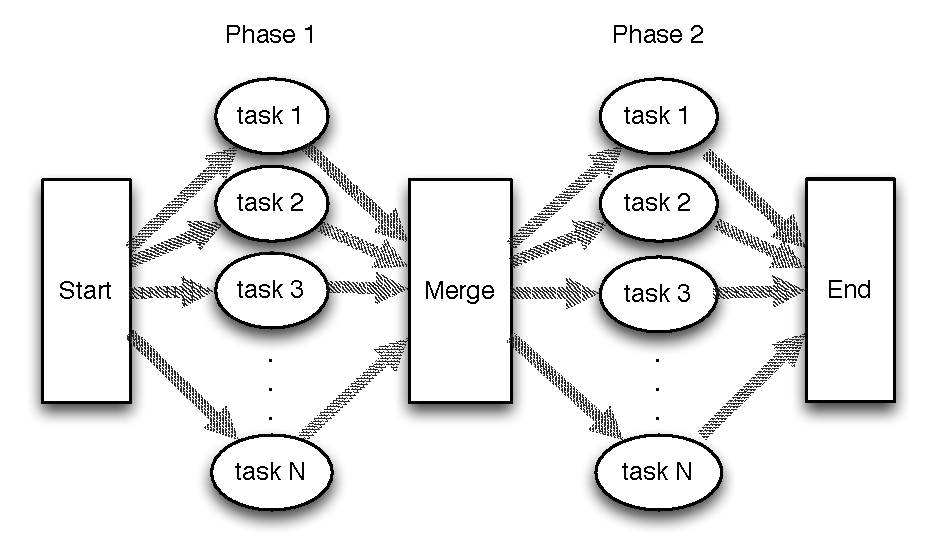
\includegraphics[width=0.6\columnwidth]{figures/system_model_1.pdf}
	\end{center}
	\caption{Cloud computing execution model with 2 phases.}
	\label{fig:system_model}
\end{figure} 

%Each task is mapped to one compute core and executes at a speed, $\sigma$. The partition of the job among tasks is
%such that each task processes a similar
%workload, $W$. Consequently, baring failures, tasks are expected to
%complete at about the same time. Therefore, the minimal response time
%of each task, when no failure occurs, is
%$t_{min}~=~\frac{W}{\sigma_{max}}$, where $\sigma_{max}$ is the maximum speed. This is also the minimal response
%time of the entire phase. 
%
%As the number of tasks increases, however, the likelihood of a task
%failure during an execution of a given phase increases
%accordingly. This underscores the importance of an energy-efficient
%fault-tolerance model to mitigate the impact of a failing task on the
%overall delay of the execution phase. Lazy Shadowing is a perfect match for the needs. We can easily apply 
%Lazy Shadowing by issuing one main and shadow pair for each task, and the execution can be performed phase 
%by phase, just as previously described. 

\section{Optimization framework}

In this section, we describe a profit-based optimization framework for
the cloud-computing execution model previous described. Using this
framework we compute profit-optimized execution speeds by
optimizing the following objective function:


\begin{equation}
\label{optimization_problem}
%\setlength{\abovedisplayskip}{14pt}
\begin{alignedat}{2}
\max_{\sigma_m,\sigma_b,\sigma_a}     & E[profit] \\
s.t.                                 & 0 \leq \sigma_m \leq \sigma_{max} \\
                                     & 0 \leq \sigma_b \leq \sigma_{m} \\
                                     & 0 \leq \sigma_a \leq \sigma_{max} 
\end{alignedat}
\end{equation}
We assume that processor
speeds are continuous and use nonlinear optimization techniques
to solve the above optimization problem. 

In order to earn profit, service providers must either increase
income or decrease expenditure. We take both factors into
consideration for the purpose of maximizing profit while meeting
customer's requirements. In our model, we set the expected profit to be
expected income minus expected expense. To model the expected income and expected expense, we built models for job reward, process failure distribution, power consumption, and energy cost. Please refer to~\cite{cui_2014_closer} for more details.

\begin{equation}
E[\text{profit}]=E[\text{income}]-E[\text{expense}]
\end{equation}



%\subsection{Reward Model}
%\label{sla_reward_model}
%
%As depicted in Figure \ref{fig:reward}, customers expect that their
%job deployed on cloud finishes by a mean response time $t_{R_1}$.  As a
%return, the provider earns a certain amount of reward, denoted by R,
%for satisfying customer's requirements. However, if the job cannot be
%completed by the expected response time, the provider loses a fraction of $R$
%proportional to the delay incurred. For large delay, the profit loss may translate into a penalty that the CSP must pay to the customer. In this model, the maximum penalty $P$ is paid if the
%delay reaches or exceeds $t_{R_2}$. The four
%parameters, $R$, $P$, $t_{R_1}$ and
%$t_{R_2}$, completely define the reward model.
%
%There are two facts that the service provider must take into account
%when negotiating the terms of the SLA. The first is the response time
%of the main process assuming no failure (Figure
%\ref{fig:sc_no_fail} and Figure \ref{fig:sc_shadow_fail}). This
%results in the following completion time:
%\begin{equation}
%t_c^m=W/\sigma_m
%\label{eq:tcm}
%\end{equation}
%
%If the main process fails (shown in Figure \ref{fig:sc_main_fail}), the
%task completion time by shadow process is the time of the failure,
%$t_f$, plus the time necessary to complete the remaining work.
%
%\begin{equation}
%t_c^s=t_f+\frac{W-t_f \times \sigma_b}{\sigma_a}
%\label{eq:tcs}
%\end{equation}
%
%
%\begin{figure}[t!]	
%	\begin{center}
%		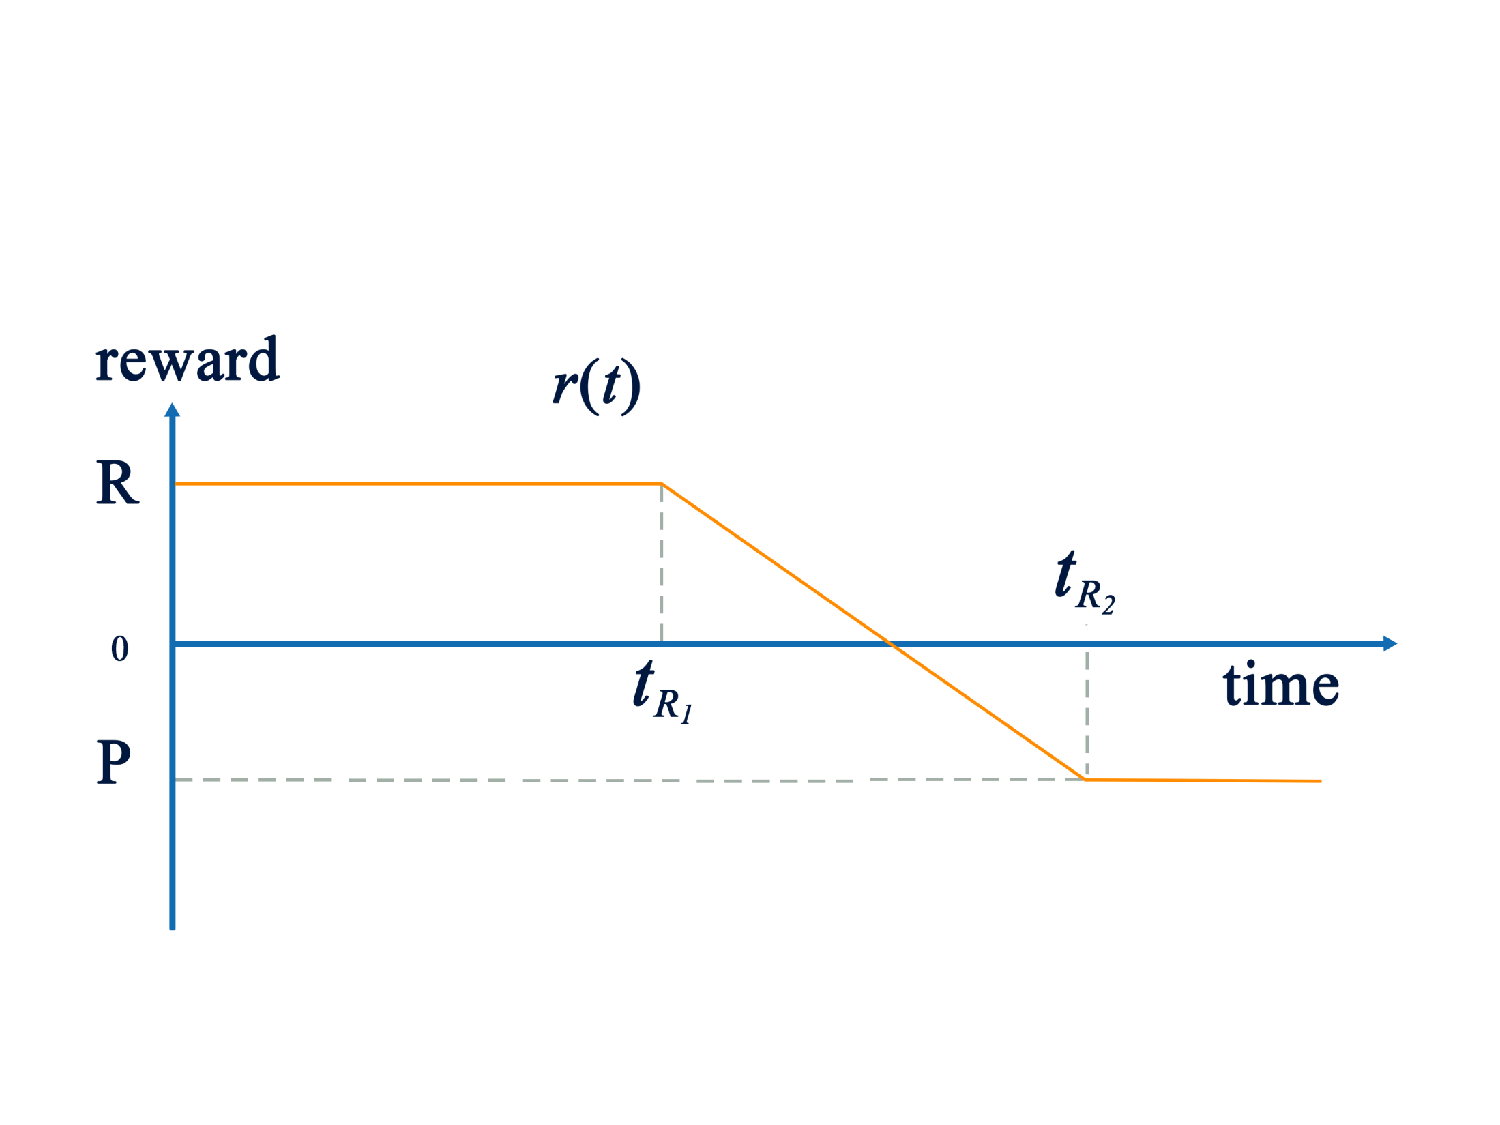
\includegraphics[width=0.6\columnwidth]{figures/reward.pdf}
%	\end{center}
%	\caption{A reward function}
%	\label{fig:reward}
%\end{figure}
%
%
%\subsection{Failure Model}
%
%We assume that two probability density functions, $f_m(t_f)$ and
%$f_s(t_f)$, exist which express the probabilities of the main and shadow
%process failing at time $t_f$ separately. The model does not assume a
%specific distribution. However, in the remainder of this paper we use
%an exponential probability density function, $f_m(t_f)=f_s(t_f)=\lambda
%e^{-\lambda t_f}$, of which the mean time between failure (MTBF) is $\frac{1}{\lambda}$.
%
%\subsection{Power and Energy Models}
%Dynamic voltage and frequency scaling
%(DVFS) has
%been widely exploited as a technique to reduce CPU dynamic power~\cite{flautner_2002_APS,pillai_2001_sosp}. It
%is well known that one can reduce the dynamic CPU power consumption at
%least quadratically by reducing the execution speed linearly. The
%dynamic CPU power consumption of a computing node executing at speed
%$\sigma$ is given by the function $p_d(\sigma)=\sigma^n$ where $n \ge
%2$.
%%% removed burd_1995_systems citation
%
%In addition to the dynamic power, CPU leakage and other components
%(memory, disk, network etc.) all contribute to static power
%consumption, which is independent of the CPU speed. We
%define static power as a fixed fraction of the node power consumed
%when executing at maximum speed, referred to as $\rho$. Hence node
%power consumption is expressed as
%$p(\sigma)=\rho \times \sigma_{max}^n + (1-\rho)\times \sigma^n$. When the execution speed is zero
%the machine is in a sleep state, powered off or not assigned as a
%resource; therefore it will not be consuming any power, static or
%dynamic.  Throughout this thesis we assume that dynamic power is cubic
%in relation to
%speed~\cite{rusu_2003_ecs,zhai_2004_dac}, therefore the
%overall system power when executing at speed $\sigma$ is defined as:
%
%\begin{equation}
%p(\sigma) = \begin{cases} \rho \sigma_{max}^3 + (1-\rho) \sigma^3 & \mbox{if } \sigma > 0 \\ 
%                          0 & \mbox{if } \sigma = 0 \end{cases}
%\label{eq:power_model}
%\end{equation}
%%% I removed chen_2012_srds from speed citation to save space
%
%Using the power model given by \ref{eq:power_model}, the
%energy consumed by a process executing at speed $\sigma$ during an
%interval $T$ is given by
%\begin{equation}
%E(\sigma,T) = p(\sigma) \times T
%\end{equation}
%
%Corresponding to \ref{fig:sc_overview}, there are three
%failure cases to consider: main and shadow both succeed, shadow fails
%and main fails. As described earlier, the case of both the main and
%shadow failing is very rare and will be ignored. The expected
%energy consumption for a single task is then the weighted average of
%the expected energy consumption in the three cases.
%
%First consider the case where no failure occurs and the main process
%successfully completes the task at time $t_c^m$, corresponding to
%\ref{fig:sc_no_fail}.
%\begin{equation}
%\begin{split}
%E_1 = &  ( 1-\int_0^{t_c^m}f_m(t)dt) \times (1 - \int_0^{t_c^m} f_s(t)dt) \times \\
%      &  (  E(\sigma_m,t_c^m) + E(\sigma_b,t_c^m))
%\label{eq:energy_no_failure}
%\end{split}
%\end{equation}
%The first line is the probability of fault-free execution of the main
%process and shadow process. Then we multiple this probability by the
%energy consumed by the main and the shadow process during this fault
%free execution, ending at $t_c^m$.
%
%Next, consider the case where the shadow process fails at some point
%before the main process successfully completes the task, corresponding to
%\ref{fig:sc_shadow_fail}.
%\begin{equation}
%\begin{split}
%E_2 = & (1-\int_0^{t_c^m}f_m(t)dt) \times \\
%      & \int_0^{t_c^m}(E(\sigma_m,t_c^m)+E(\sigma_b,t)) \times f_s(t)dt
%\label{eq:energy_shadow_fail}
%\end{split}
%\end{equation}
%The first factor is the probability that the main process does not
%fail, and the probability of shadow fails is included in the second factor which also contains the energy consumption since it depends on the shadow failure time. Energy consumption comes from the main process until the completion of the task,
%and the shadow process before its failure.
%
%The one remaining case to consider is when the main process fails and
%the shadow process must continue to process until the task completes,
%corresponding to Figure \ref{fig:sc_main_fail}.
%\begin{equation}
%\begin{split}
%E_3 = & (1-\int_0^{t_c^m}f_s(t)dt) \times \int_0^{t_c^m}(E(\sigma_m,t)+\\
%      & E(\sigma_b,t)+E(\sigma_a,t_c^s-t))f_m(t)dt
%\label{eq:energy_main_fail}
%\end{split}
%\end{equation}
%Similarly, the first factor expresses the probability that the shadow process does
%not fail. In this case, the shadow process executes from the beginning to
%$t_c^s$ when it completes the task. However, under our ``at most one
%failure'' assumption, the period during which shadow process may fail
%ends at $t_c^m$, since the only reason why shadow process is still in
%execution after $t_c^m$ is that main process has already failed. There
%are three parts of energy consumption, including that of main process
%before main's failure, that of shadow process before main's failure,
%and that of shadow process after main's failure, all of which depend
%on the failure occurrence time. 
%
%The three equations above describe the expected energy consumption by a
%pair of main and shadow processes for completing a task under
%different situations. However, under our system model it might be the
%case that those processes that finish early will wait idly and
%consume static power if failure delays one task. If it is the case
%that processes must wait for all tasks to complete, then this energy
%needs to be accounted for in our model. The probability of this is the probability that at least one main process fails,
%referred to as the system level failure probability.
%\begin{equation}
%P_f=1-(1-\int_0^{t_c^m}f_m(t)dt)^N
%\label{eq:prob_of_one_main_failure}
%\end{equation}
%Hence, we have the fourth equation corresponding to the energy consumed while waiting in idle. 
%\begin{equation}
%  \begin{split}
%  E_4 = & ( 1-\int_0^{t_c^m}f_m(t)dt) \times (1 - \int_0^{t_c^m} f_s(t)dt) \times \\
%        & 2 P_f \times E(0,t_c^j-t_c^m) + \int_0^{t_c^m}f_s(t)dt \times \\
%        & (1-\int_0^{t_c^m}f_m(t)dt) \times P_f \times E(0,t_c^j-t_c^m) 
%  \end{split}
%\end{equation}
%Corresponding to the first case, neither main process nor shadow
%process fails, but both of them have to wait in idle from task
%completion time $t_c^m$ to the last task's completion (by a shadow
%process) with probability $P_f$. Under the second case, only the main
%process has to wait if some other task is delayed since its shadow
%process has already failed. These two aspects are accounted in the
%first and last two lines in $E_4$ separately.  We use the expected
%shadow completion time $t_c^j$ as an approximation of the latest task
%completion time which is also the job completion time.
%
%By summing these four parts and then multiplying it by $N$ we will have
%the expected energy consumed by Shadow Replication for completing a
%job of $N$ tasks.
%\begin{equation}
%E[\text{energy}]=N \times (E_1 + E_2 + E_3 + E_4)
%\label{eq:total_energy}
%\end{equation}
%
%\subsection{Income and Expense Models}
%The income is the reward paid by customer for the cloud computing
%services that they utilize. It depends on the reward function $r(t)$,
%depicted in \ref{fig:reward}, and the actual job completion
%time. Therefore, the income should be either $r(t_c^m)$, if all main
%processes can complete without failure, or $r^*(t_c^s)$ otherwise. It
%is worth noting that the reward in case of failure should be
%calculated based on the last completed task, which we approximate by
%calculating the expected time of completion allowing us to derive the
%expected reward, i.e. $r^*(t_c^s)=\frac{\int_0^{t_c^m}r(t_c^s) \times
%f_m(t)dt}{\int_0^{t_c^m}f_m(t)dt}$. Therefore the income is estimated
%by the following equation.
%\begin{equation}
%E[\text{income}]= (1-P_f) \times r(t_c^m) + P_f \times r^*(t_c^s)
%\end{equation}
%
%The first part is the reward earned by the main process times the
%probability that all main processes would complete tasks without
%failure. If at least one main process fails, that task would have to
%be completed by a shadow process. As a result, the second part is the
%reward earned by shadow process times the system level failure probability.
%
%If $C$ is the charge expressed as dollars per unit of energy consumption
%(e.g. kilowatt hour), then the expected expenditure would be $C$ times
%the expected energy consumption for all $N$ tasks:
%\begin{equation}
%E[\text{expense}] = C \times E[\text{energy}]
%\label{eq:expense}
%\end{equation}


\section{Profit-aware stretched replication} 
Unlike traditional replication
Shadow Replication is dependent upon failure detection, enabling the
replica to increase its execution speed upon failure and maintain the
targeted response time thus maximizing profit. While this is the case
in many computing environments, there are cases where failure
detection may not be possible. To address this limitation, we propose
profit-aware stretched replication, whereby both the main process and
the shadow execute independently at stretched speeds to meet the
expected response time, without the need for failure
detection. In profit-aware stretched replication both the main and
shadow execute at speed $\sigma_r$, found by optimizing the profit
model.  For both traditional replication and stretched replication,
the task completion time is independent of failure and can be directly
calculated as:
\begin{equation}
t_c=\frac{W}{\sigma_{max}} \text{ or } t_c=\frac{W}{\sigma_r}
\end{equation}


Since all tasks will have the same completion time, the job completion
time would also be $t_c$. Further, the expected income, which depends
on negotiated reward function and job completion time, is independent
of failure:
\begin{equation}
E[income]=r(t_c)
\end{equation}

Since both traditional replication and profit-aware stretched
replication are special cases of our Shadow Replication paradigm where
$\sigma_m=\sigma_b=\sigma_a=\sigma_{max}$ or
$\sigma_m=\sigma_b=\sigma_a=\sigma_r$ respectively, we can easily derive the
expected energy consumption using \ref{eq:total_energy} with $E_4$
fixed at 0 and then compute the expected expense using \ref{eq:expense}.

\section{Re-execution}

\noindent 
Contrary to replication, re-execution initially assigns a single
process for the execution of a task. If the original task fails, the
process is re-executed. In the cloud computing execution framework
this is equivalent to a checkpoint/restart, the checkpoint is
implicitly taken at the end of each phase and because the tasks are
loosely coupled they can restart independently. 

Based on the one failure assumption, two cases must be considered to
calculate the task completion time. If no failure occurs, the task
completion time is:
\begin{equation}
t_c=\frac{W}{\sigma_{max}}
\end{equation}
In case of failure, however, the completion time is equal to the sum
of the time elapsed until failure and the time needed for
re-execution. Again, we use the expected value
$t_f^*=\frac{\int_0^{t_c}t \times f_m(t)dt}{\int_0^{t_c}f_m(t)dt}$ to
approximate the time that successfully completed processes have to
spend waiting for the last one.

Similar to Shadow Replication, the income for re-execution is the
weighted average of the two cases:
\begin{equation}
E[\text{income}]=(1-P_f) \times r(t_c) + P_f \times r(t_c+t_f^{*})
\end{equation}

For one task, if no failure occurs then the expected energy consumption can be
calculated as
\begin{equation}
E_5=(1 - \int_0^{t_c} f_m(t)dt) \times (E(\sigma_{max},t_c)+ P_f \times E(0,t_f^{*}))
\label{eq:energy_first_task}
\end{equation}

If failure occurs, however, the expected energy consumption can be calculated
as
\begin{equation}
E_6=\int_0^{t_c}(E(\sigma_{max},t) + E(\sigma_{max},t_c)) \times f_m(t) dt
\label{eq:energy_rexecution_task}
\end{equation}
Therefore, the expected energy consumption by re-execution for
completing a job of $N$ tasks is
\begin{equation}
E[energy]=N \times (E_5 + E_6)
\end{equation}

\section{Performance evaluation}

This section evaluates the expected profit of each of the fault tolerance
methods discussed above under different system environment. We have identified 5
important parameters which affect the expected profit:
\begin{itemize}
\item Static power ratio $\rho$, which determines the portion of power that is unaffected by the execution speed.
\item SLA - The amount of reward, penalty and the required response times.
\item $N$ - The total number of tasks.
\item MTBF - The reliability of an individual node.
\item Workload - The size, $W$, of each individual task.
\end{itemize}


Without loss of generality, we normalize $\sigma_{max}$ to be 1, so
that all the speeds can be expressed as a fraction of maximum
speed. Accordingly, the task workload $W$ is also adjusted such that
it is equal to the amount of time (in hours) required for a single
task, preserving the ratios expressed in
\ref{eq:tcm} and \ref{eq:tcs}. The price of
energy is assumed to be 1 unit. We assume that $R$ in our reward model
is linearly proportional to the number of tasks $N$ and the maximal
reward for one task is 3 units, so the total reward for a job is $3
\times N$ units.  However, for the analysis we look
at the average of expenditure and income on each task by dividing the
total expenditure and income by $N$. In our basic configuration we
assume that the static power ratio is 0.5, the task size is 1 hour, the node MTBF 5 is
years, the number of tasks is $100000$, and the response time thresholds for
maximal and minimal rewards are 1.3 hours and 2.6 hours
respectively. Since the maximal power consumption is 1 unit, the
energy needed for the task with one process at maximal speed is also 1
unit. 


With various architectures and organizations, servers deployed at
different data centers will have different characteristics in terms of
power consumption. The static power ratio is used to abstract the
amount of static power consumed versus dynamic power.  

\begin{figure}[!h]	
	\begin{center}
		\subfigure[Profit for different static power ratio. MTBF=5 years, N=100000, W=1 hour, $t_{R_1}$=1.3 hours, $t_{R_2}$=2.6 hours.]
		{
			\label{fig:rho}
			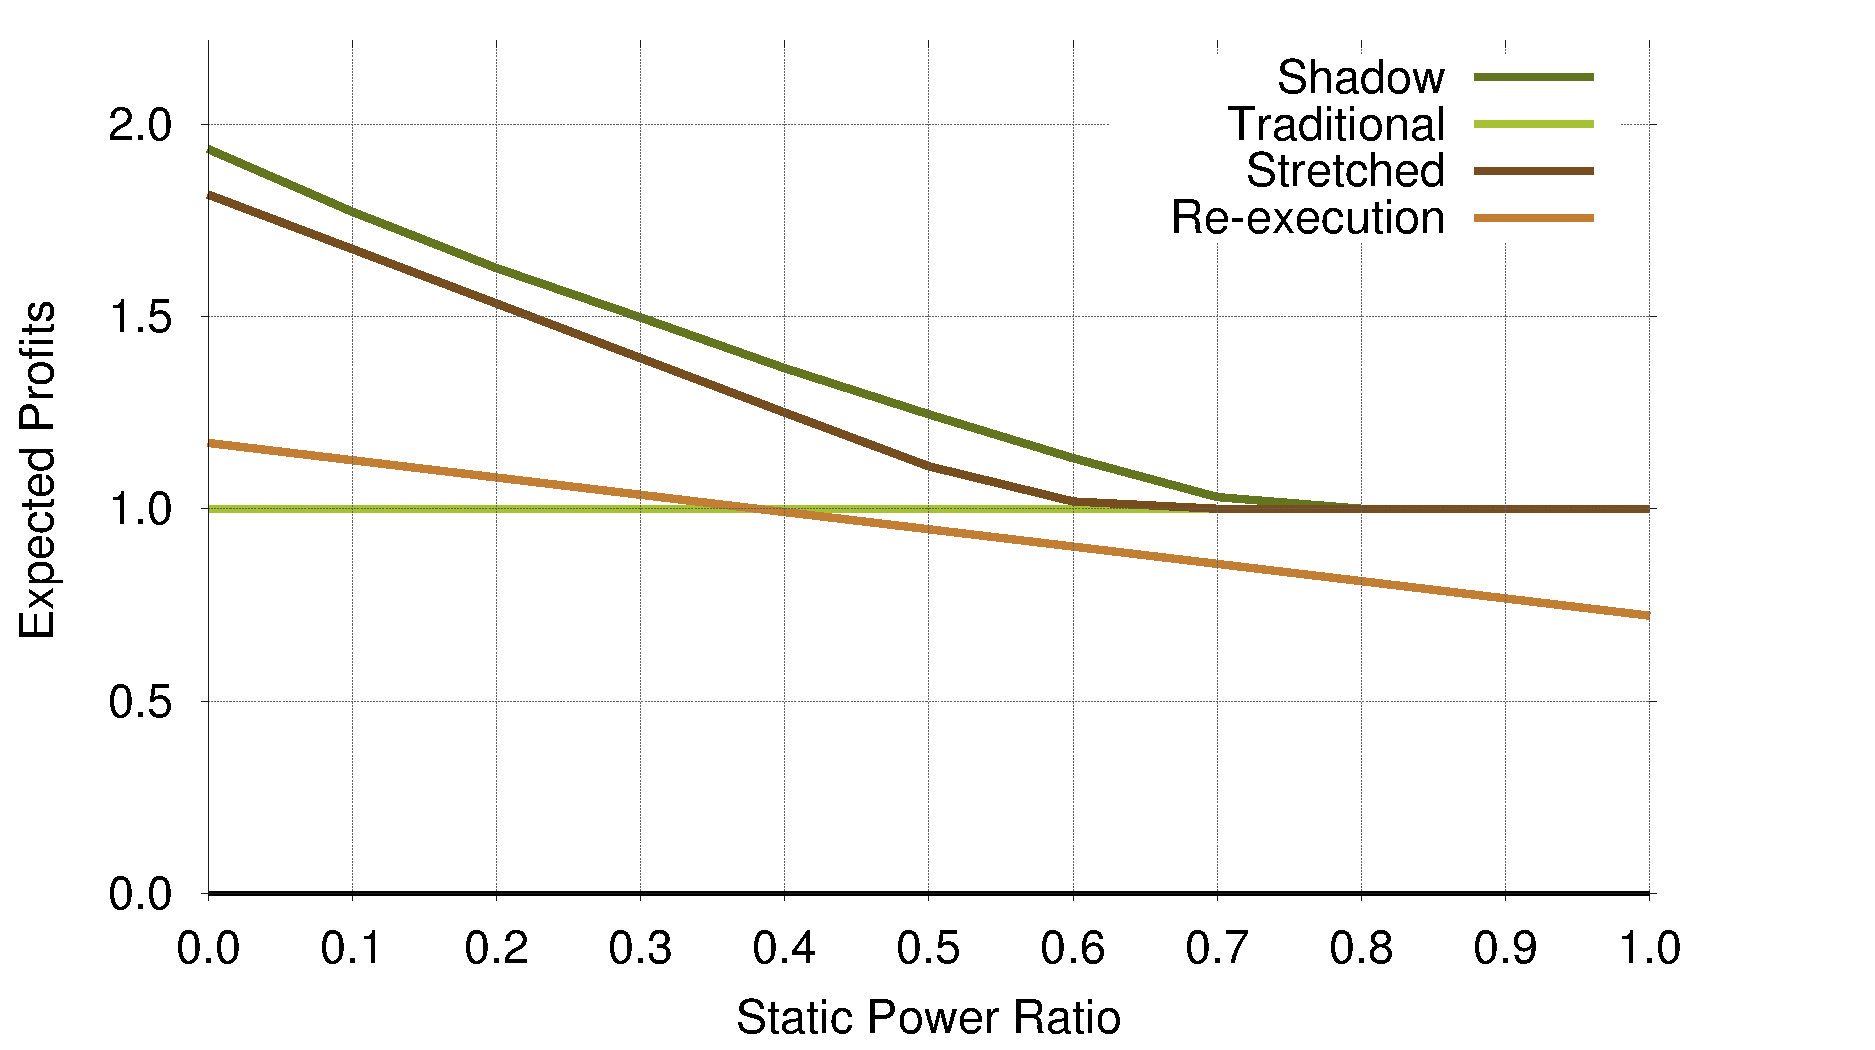
\includegraphics[width=0.4\columnwidth]{figures/rho_profit.pdf}
		}
		\subfigure[Profit for different response time threshold. $\rho$=0.5, MTBF=5 years, N=100000, W=1 hour.]
		{
			\label{fig:t}
			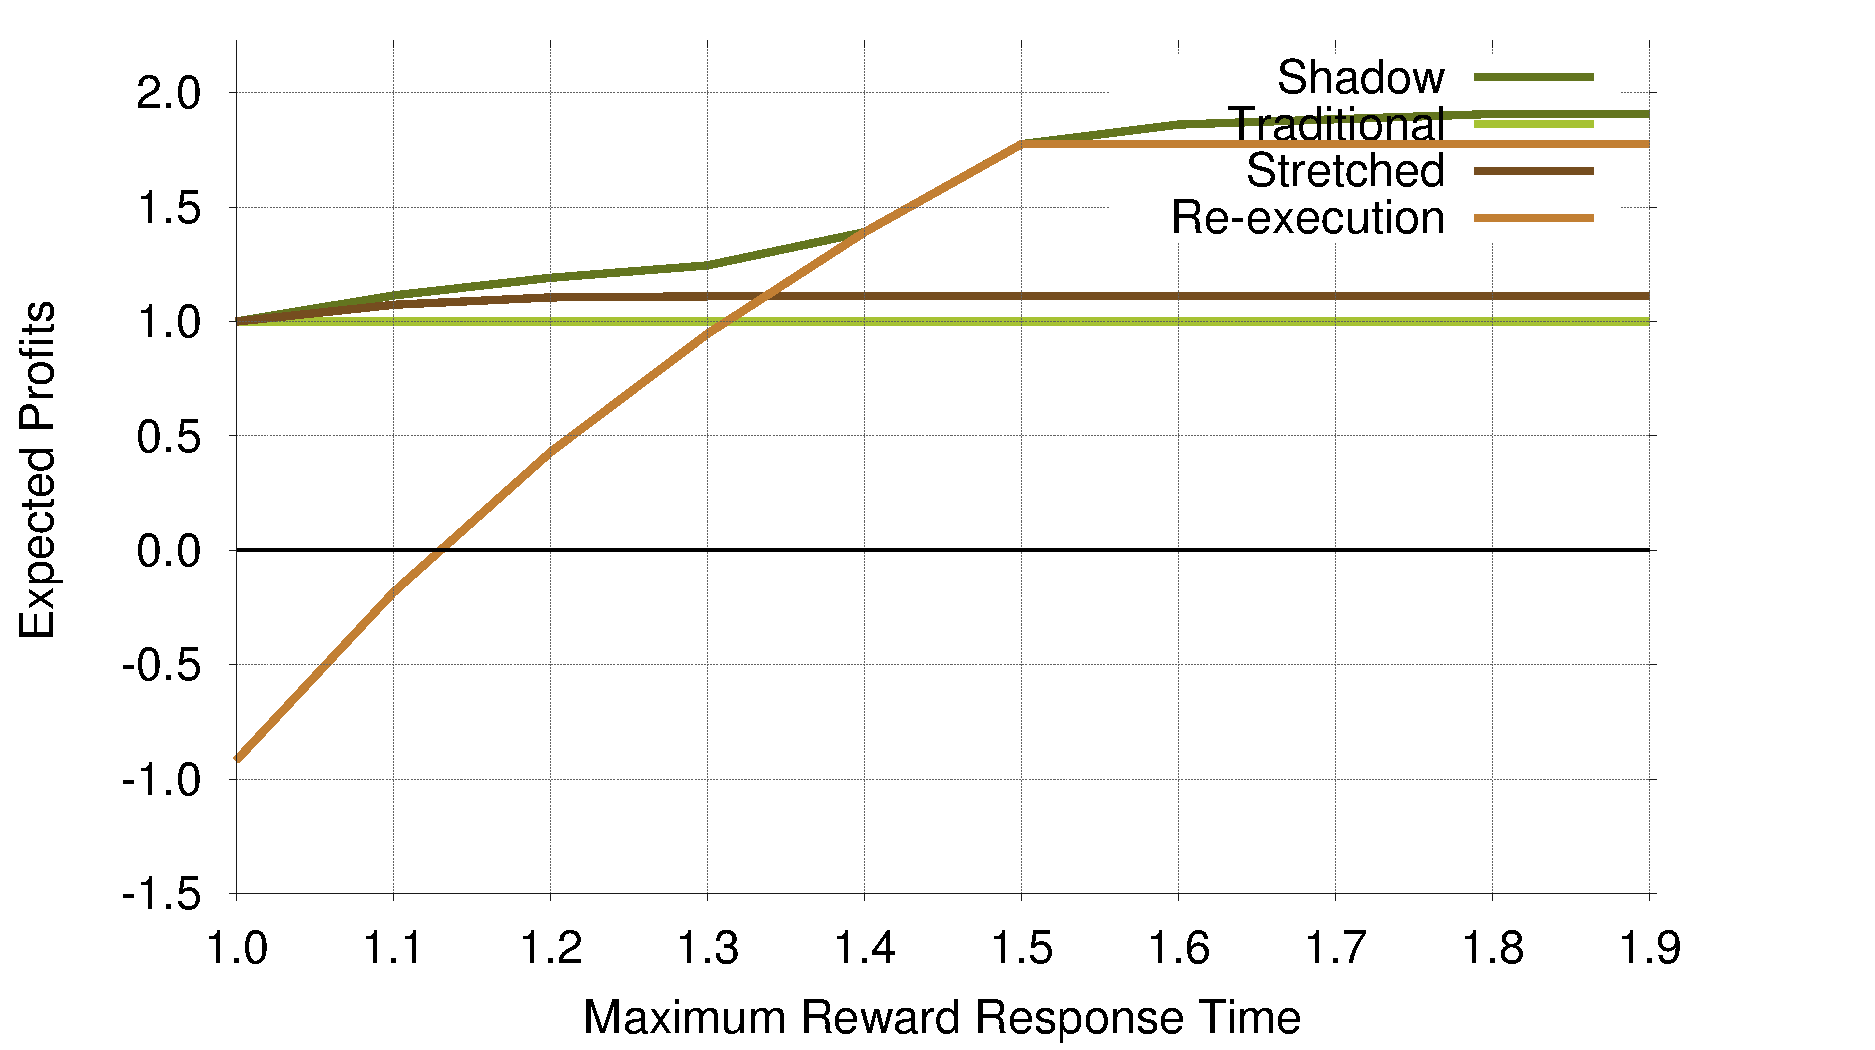
\includegraphics[width=0.4\columnwidth]{figures/t_profit.pdf}
		}
		\subfigure[Profit for different task size over MTBF. $\rho$=0.5, N=100000, $t_{R_1}$=1.3 hours, $t_{R_2}$=2.6 hours.]
		{
			\label{fig:n}
			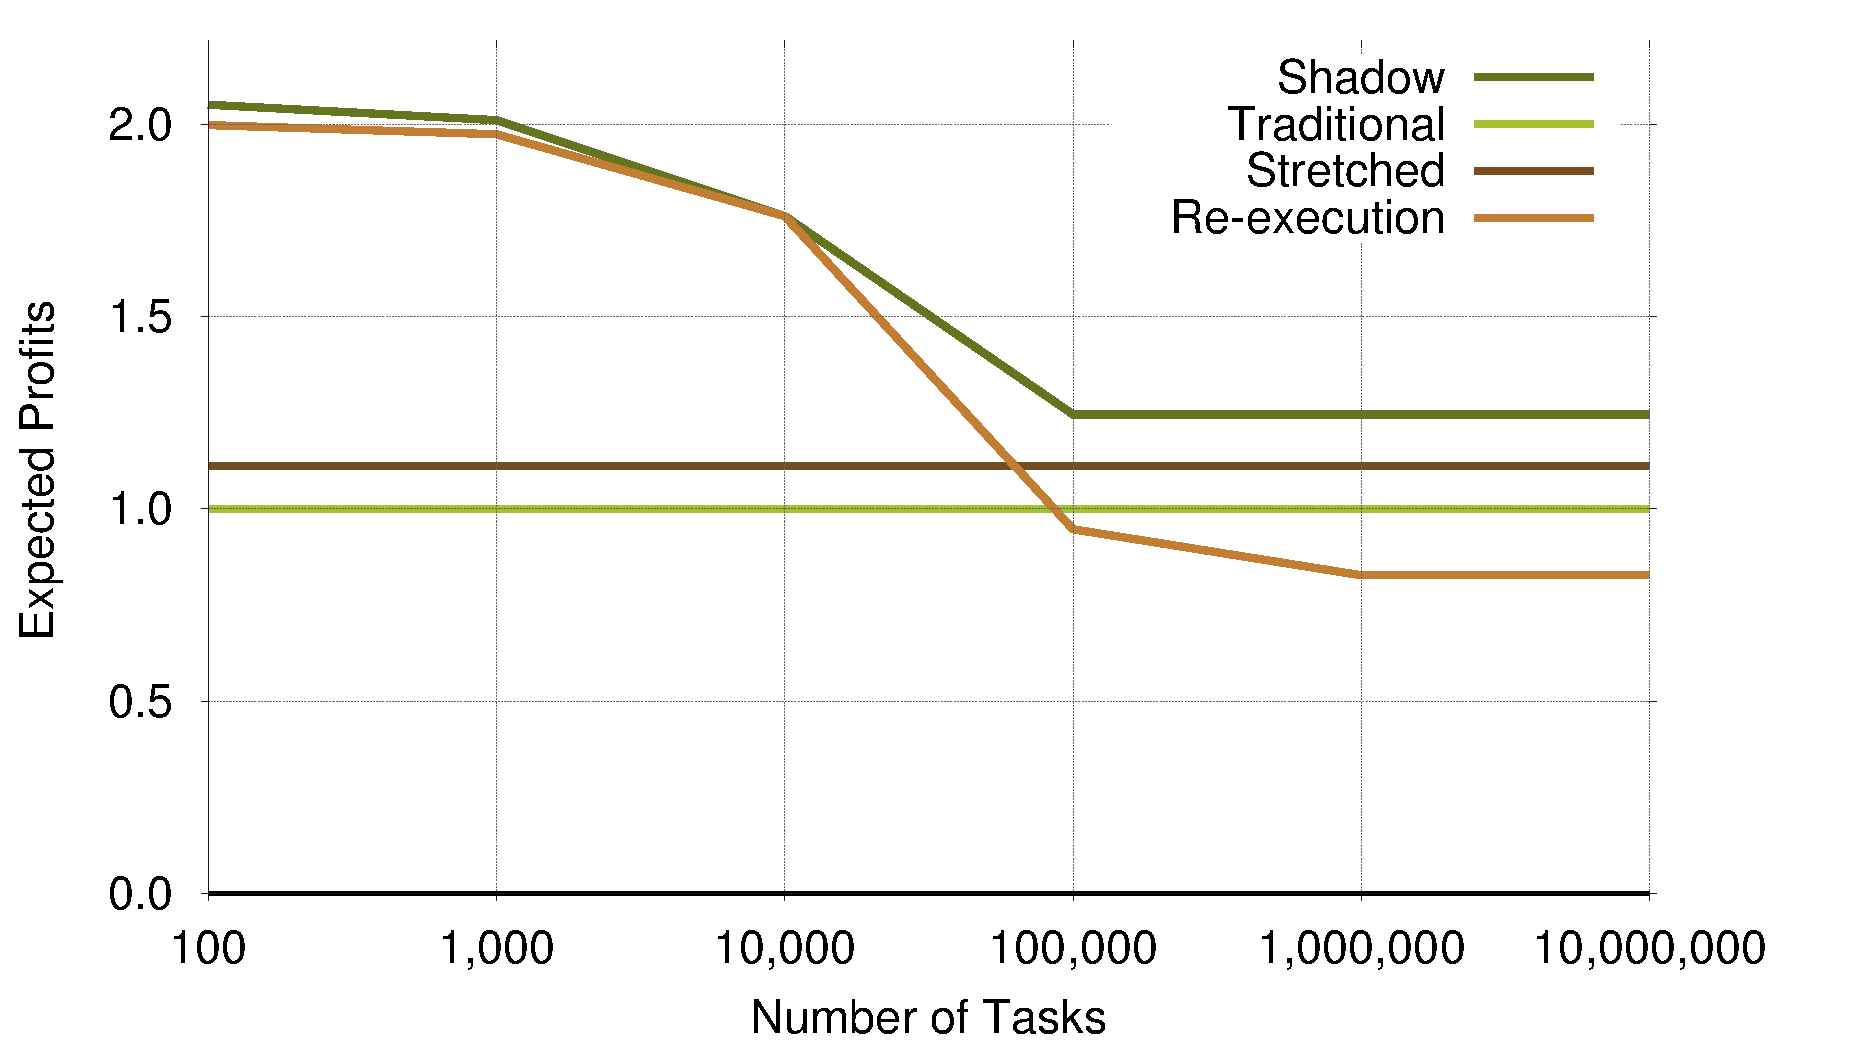
\includegraphics[width=0.4\columnwidth]{figures/n_profit.pdf}
		}
		\subfigure[Profit for different task size over MTBF. $\rho$=0.5, N=100000, $t_{R_1}$=1.3 hours, $t_{R_2}$=2.6 hours.]
		{
			\label{fig:mtbf}
			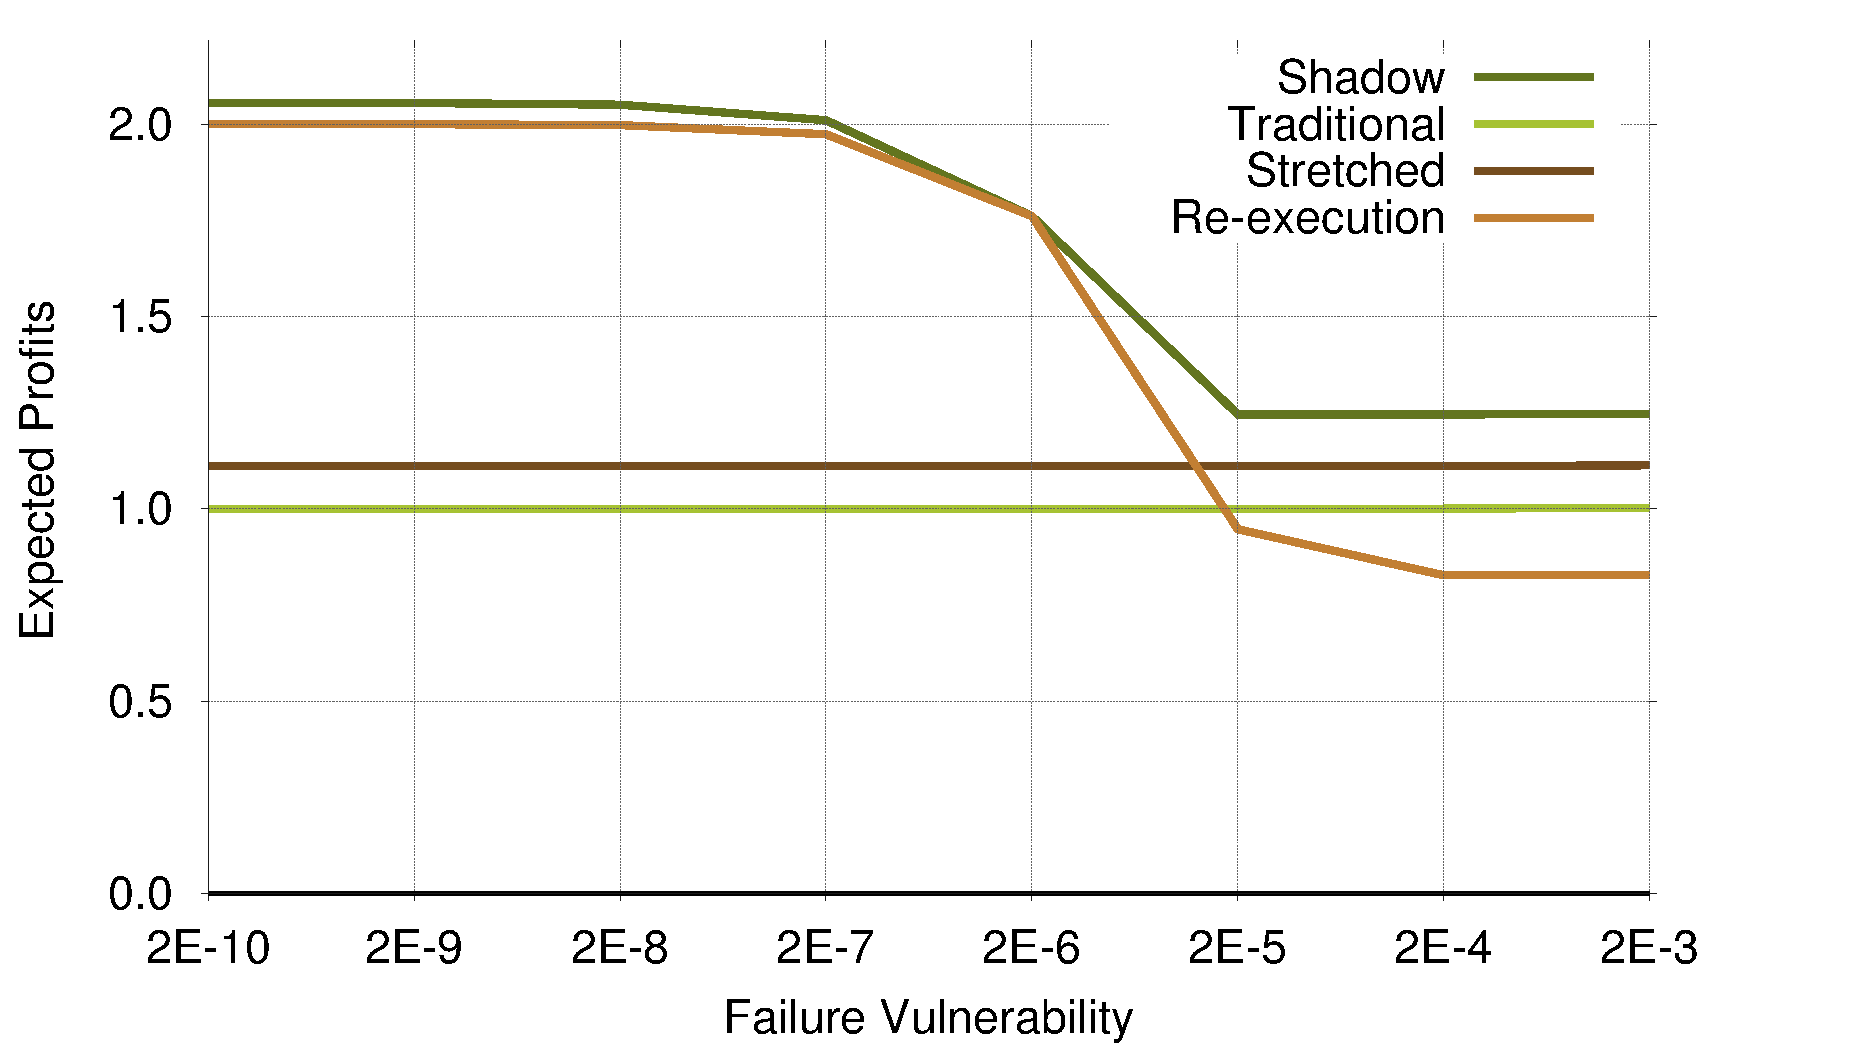
\includegraphics[width=0.4\columnwidth]{figures/mtbf_profit.pdf}
		}
	\end{center}

\end{figure}


The potential profit gains achievable by using profit-aware
replication techniques decreases as static power increases, as is shown
in Figure~\ref{fig:rho}. The reason is that our profit-aware
techniques rely upon the fact that one can reduce energy costs by
adjusting the execution speeds. Modern systems have a static power between 40\%-70\% and
it is reasonable to suspect that this will continue to be the case. Within
this target range of static power, Shadow Replication can achieve, on
average, 19.3\% more profit than traditional replication, 8.9\% more
than profit-aware stretched replication, and 28.8\% more than re-execution.

Figure~\ref{fig:t} shows the effect that targeted response time has upon
the profitability of each fault tolerance method. We vary the first threshold $t_{R_1}$ from the minimal response
time $t_{min}$ to $1.9t_{min}$, and set the second threshold $t_{R_2}$
to be always $2t_{R_1}$. Compared to traditional replication, all the other methods increase their profit as the targeted
response time increases, this is expected because each of the other
techniques can make use of increased laxity in time to increase
profit. Re-execution is the most sensitive to the target response
time since it fully relies upon time redundancy, showing that it should only be used when the targeted response time is \emph{not} stringent. 
Again, Shadow Replication always achieves more profit than traditional
replication and profit-aware stretched replication, and the profit
gains are 52.8\% and 39.0\% on average. 

Figure \ref{fig:n} confirms that for small number of tasks
re-execution is more profitable than replication. However, re-execution is not scalable
as its profit decreases rapidly after N reaches 10000. At the same time, traditional
replication and profit-aware stretched replication are not
affected by the number of tasks because neither are affected by the
system level failure rate. On average, Shadow Replication achieves 43.5\%, 59.3\%, and 18.4\%
more profits than profit-aware stretched replication, traditional replication and re-execution, respectively. 

The ratio between task size and node MTBF represents the tasks
vulnerability to failure, specifically it is an approximation of the
probability that failure occurs during the execution of the task. In our
analysis we found that increasing task size will have the same effect
as reducing node MTBF. Therefore, we analyze these together using the
vulnerability to failure, allowing us to analyze a wider range of
system parameters. As expected
re-execution is desired when the vulnerability to failure is
low. As always, Shadow Replication can adjust its execution strategy to maximize the profits, as shown in Figure~\ref{fig:mtbf}.

Lastly, we evaluate
the expected profit of each resilience technique using three different
benchmark applications representing a wide range of
application~\cite{mrbs}: Business Intelligence, Bioinformatics and
Recommendation System. 
Using the results of the experiments reported in \cite{mrbs}, we
derived that the time required to process data for above application types are 3.3 MB/s, 6.6 MB/s, and 13.2 MB/s, respectively. 

\begin{figure}[!h]
	
	\begin{center}
	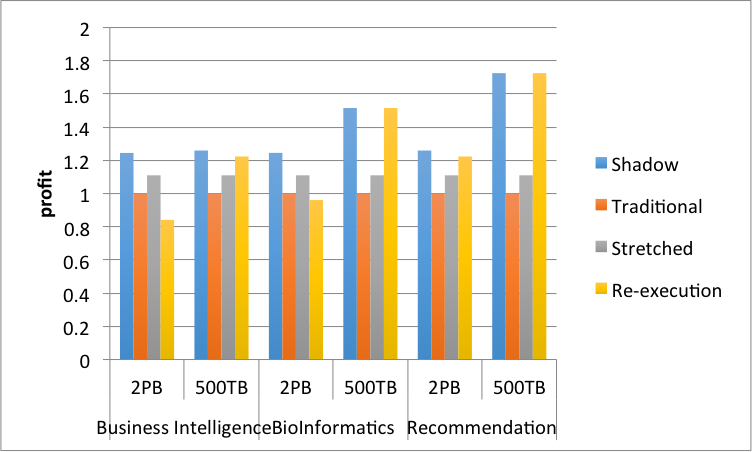
\includegraphics[width=\columnwidth]{figures/application_comparison.png}
	\end{center}
	\caption{Application comparison. $\rho$=0.5, N=$500000$, $t_{R_1}$=$1.3t_{min}$, $t_{R_2}$=$2.6t_{min}$.}
	\label{fig:app_compare}
\end{figure}


In Figure \ref{fig:app_compare} we compare the expected
profit for each application using each of the 4 resilience techniques. 
We consider two data sizes expected in future
cloud computing environments, 500TB and 2PB. The figure shows that
for business intelligence applications, Shadow Replication achieves significantly larger profits for both data sizes. This
is because business intelligence applications tend to be IO intensive
resulting in longer running tasks. Whereas recommendation systems tend
to require little data IO resulting in shorter running tasks making
re-execution as good as Shadow Replication. Bioinformatics tends to be in between
these two applications resulting in shadow computing performing better
when processing large datasets (2 PB) but not outstanding on smaller
datasets (500 TB). The take away from this evaluation is that for the
shown system parameters if phase execution is short, then re-execution
performs as well as Shadow Replication. Alternatively, if a phase is long (20 minutes or
greater), then Shadow Replication can be as much as 47.9\% more
profitable than re-execution. The previous sensitivity analysis can be
used to extrapolate expected profit for different system parameters.

\section{Summary}

To assess the performance of the Lazy Shadowing, an analytical framework is developed and 
an extensive performance evaluation study is carried out. 
In this study, system properties that affect the
profitability of fault tolerance methods, namely failure rate,
targeted response time and static power, are identified. The failure rate is
affected by the number of tasks and vulnerability of the task
to failure. The targeted response time represents the 
clients' desired job completion time.  
Our performance evaluation shows that in all cases, Shadow Replication outperforms
existing fault tolerance methods. Furthermore, shadow
replication will converge to traditional replication when target response time is stringent, and to re-execution when target response time is relaxed or failure is unlikely.


   




